% ==============================================================================
% SECCION 4: ACTIVIDAD 3 - FUGAS, RETENCION Y DIMENSIONAMIENTO DEL KEEPER
% ==============================================================================
\section{Actividad 3: Fugas, Retención y Dimensionamiento del Keeper}
\label{sec:actividad3}

En tecnologías nanométricas sub-45\,nm, el adelgazamiento del óxido de compuerta ($t_{oxe} = 1.25\,\text{nm}$) y la reducción de las tensiones de umbral incrementan exponencialmente las corrientes de fuga parásitas. En lógica CMOS dinámica, estas fugas descargan progresivamente el nodo dinámico cuando el reloj se detiene en evaluación (\textit{clock gating} para ahorro de energía), induciendo conmutaciones lógicas erróneas si no se incorpora un circuito de compensación (\textit{keeper}). Esta sección aborda la caracterización cuantitativa de las componentes de fuga, su dependencia térmica, la comparación tecnológica tri-nodo y el compromiso de diseño entre retención y penalización de velocidad.

\subsection{Retención del Nodo Dinámico y Pérdida de Carga en Evaluación}
Para evaluar la inmunidad al apagado del reloj, se implementó el protocolo de retención estipulado en la guía (§7): con $V_{DD} = 1.0\,\text{V}$, las entradas se fijan estáticamente en $A=B=C=0$ (PDN abierta), mientras la señal de reloj conmuta a nivel alto en $t_{\text{eval\_start}} = 0.52\,\text{ns}$ y permanece detenida en evaluación durante $T_{\text{ret}} = 1.0\,\mu\text{s}$ (hasta el tiempo final de simulación $T_{\text{stop}} = 1000.52\,\text{ns}$). En esta condición, el transistor de precarga $M_p$ se encuentra cortado ($V_{GS} = 0\,\text{V}$), dejando al nodo $dyn$ en estado flotante.

\begin{figure}[htbp]
  \centering
  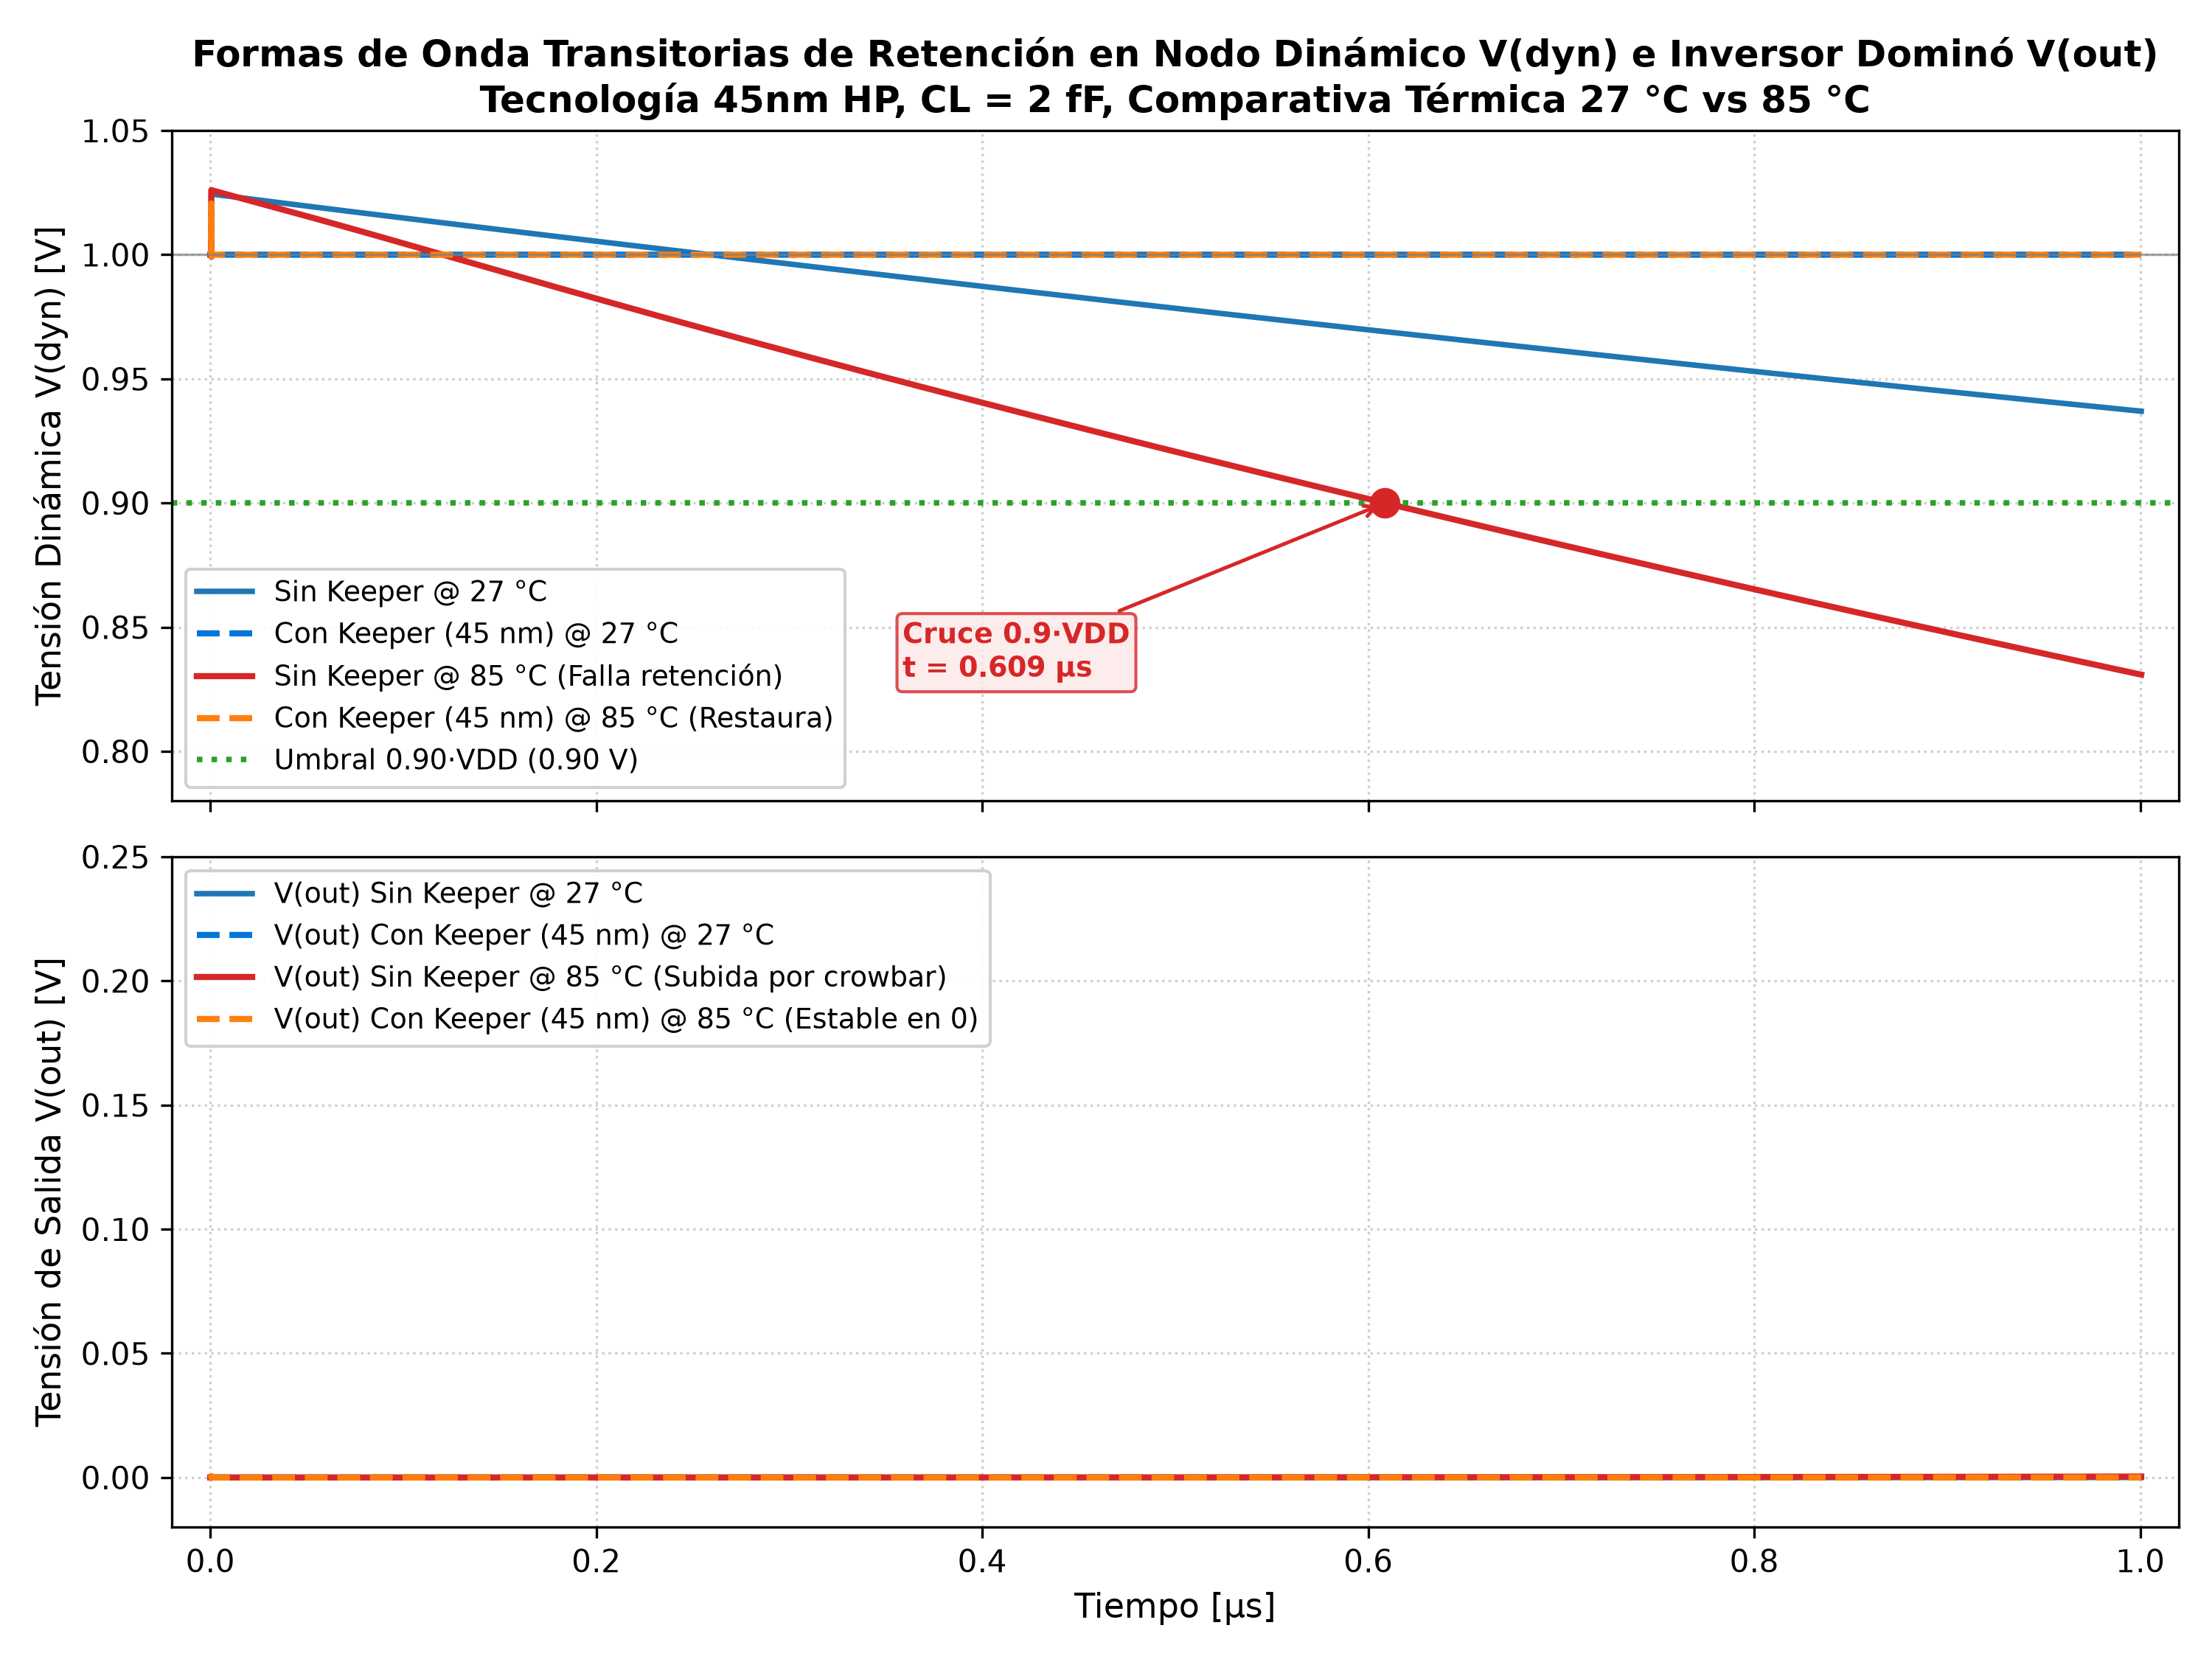
\includegraphics[width=0.62\linewidth]{figuras/fig1_act3_retencion_formas_onda.png}
  \caption[Formas de onda transitorias de retención en el nodo dinámico]{Formas de onda transitorias de retención en el nodo $dyn$ y salida $out$ durante $1.0\,\mu\text{s}$ en 45\,nm HP ($C_L=2\,\text{fF}$), contrastando la respuesta sin keeper a $27^\circ\text{C}$ y $85^\circ\text{C}$ frente al circuito con keeper ($W_{kp}=45\,\text{nm}$).}
  \label{fig:retencion_formas_onda}
\end{figure}

Las curvas transitorias se presentan en la Figura~\ref{fig:retencion_formas_onda}. En ausencia de keeper:
\begin{itemize}[leftmargin=1.4em,itemsep=0.15em]
  \item \textbf{A temperatura ambiente ($27^\circ\text{C}$):} La tensión dinámica evoluciona entre los extremos medidos $V_{dyn}(t_0 = 10.0\,\text{ns}) = 1.023497\,\text{V}$ y $V_{dyn}(t_1 = 1000.520\,\text{ns}) = 0.936959\,\text{V}$, registrando una caída total de $\Delta V_{dyn} = -86.538\,\text{mV}$. El circuito \textbf{cumple holgadamente} el criterio estricto de la guía ($V_{dyn} > 0.90\,V_{DD} = 0.90\,\text{V}$) durante todo el intervalo de $1\,\mu\text{s}$.
  \item \textbf{A alta temperatura ($85^\circ\text{C}$):} El incremento térmico de las corrientes de fuga acelera el drenaje de portadores, con extremos reales $V_{dyn}(t_0) = 1.023977\,\text{V}$ y $V_{dyn}(t_1) = 0.830869\,\text{V}$ ($\Delta V_{dyn} = -193.108\,\text{mV}$). La tensión cruza el umbral de $0.90\,V_{DD} = 0.90\,\text{V}$ en un tiempo absoluto transitorio de $t_{\text{cross}} = 608.69\,\text{ns}$, lo que equivale a un tiempo de retención neto en evaluación de $t_{\text{hold}} = t_{\text{cross}} - t_{\text{eval\_start}} = 608.17\,\text{ns}$ (con $t_{\text{eval\_start}} = 0.52\,\text{ns}$), \textbf{incumpliendo el criterio estricto de retención} frente a la ventana de evaluación ensayada de $1.0\,\mu\text{s}$ ($T_{\text{ret}} = 1000.0\,\text{ns}$). No obstante, dado que $V_{dyn}(1\,\mu\text{s}) = 0.831\,\text{V}$ se mantiene por encima de la tensión de conmutación del inversor dominó ($V_M \approx 0.50\,\text{V}$), la salida permanece estable en $out = 0\,\text{V}$, sin manifestar falla lógica funcional dentro de la ventana de $1\,\mu\text{s}$.
\end{itemize}

\noindent\textbf{Acoplamiento Capacitivo en $t_0$:} En ambas temperaturas, $V_{dyn}(t_0)$ supera ligeramente la tensión de alimentación nominal ($1.0235\,\text{V}$ y $1.0240\,\text{V}$). Este fenómeno responde al acoplamiento capacitivo (\textit{clock feedthrough} / \textit{bootstrap}) transmitido por la capacitancia de solapamiento compuerta-drenaje $C_{gd}(M_p)$ durante la transición ascendente del reloj ($CLK: 0 \to 1\,\text{V}$); por ende, no debe asumirse artificialmente $V_{dyn}(t_0) = 1.000\,\text{V}$.

\subsubsection{Conciliación Metodológica de Capacitancias Nodal y Aparente}
En la formulación analítica previa se estimó una capacitancia parásita estática en pequeña señal de $C_{\text{par}} \approx 0.65\,\text{fF}$, resultando en $C_{dyn,\text{teor}} \approx C_L + C_{\text{par}} \approx 2.65\,\text{fF}$. Sin embargo, la integración numérica directa en gran señal revela una dinámica aparente distinta:
\begin{enumerate}[leftmargin=1.4em,itemsep=0.12em]
  \item \textbf{Parámetro circuital explícito ($C_L = 2.0\,\text{fF}$):} La integración temporal de la corriente terminal $I(C_L)$ en el archivo RAW durante la ventana $\Delta t = 990.520\,\text{ns}$ arroja $\langle I(C_L) \rangle = -174.732\,\text{pA}$ a $27^\circ\text{C}$ y $-389.913\,\text{pA}$ a $85^\circ\text{C}$, coincidente a seis cifras significativas con $C_L \frac{\Delta V_{dyn}}{\Delta t}$. El capacitor físico concentra el 91.5\% de la corriente total de descarga.
  \item \textbf{Capacitancia dinámica aparente inferida ($C_{\text{eff}}$):} A partir del balance integral de cargas con la corriente terminal neta demandada por los semiconductores ($\langle I_{\text{net,dev}} \rangle$):
  \begin{equation}
    C_{\text{eff}} \equiv \frac{\langle I_{\text{net,dev}} \rangle \cdot \Delta t}{|\Delta V_{dyn}|} = 
    \begin{cases}
      \dfrac{191.021\,\text{pA} \times 990.520\,\text{ns}}{86.53768\,\text{mV}} = \mathbf{2.18645\,\text{fF}} & (27^\circ\text{C}) \\[1em]
      \dfrac{425.281\,\text{pA} \times 990.520\,\text{ns}}{193.10813\,\text{mV}} = \mathbf{2.18142\,\text{fF}} & (85^\circ\text{C})
    \end{cases}
    \label{eq:ceff}
  \end{equation}
  \item \textbf{Capacitancia parásita aparente ($C_{\text{par}}$):} Se deduce algebraicamente para cerrar la ley de Kirchhoff:
  \begin{equation}
    C_{\text{par,aparente}} \equiv C_{\text{eff}} - C_L = 
    \begin{cases}
      0.18645\,\text{fF} & (27^\circ\text{C}) \\
      0.18142\,\text{fF} & (85^\circ\text{C})
    \end{cases}
  \end{equation}
  suministrando el remanente dinámico de $+16.29\,\text{pA}$ a $27^\circ\text{C}$ y $+35.37\,\text{pA}$ a $85^\circ\text{C}$.
\end{enumerate}

\noindent\textbf{Interpretación Física Plausible:} La reducción de la capacitancia parásita efectiva frente a la predicción estática lineal ($0.186\,\text{fF}$ vs $0.65\,\text{fF}$) se fundamenta en las condiciones de polarización dinámica durante la retención:
\begin{itemize}[leftmargin=1.4em,itemsep=0.1em]
  \item Al mantenerse $V_{dyn} \approx 1.0\,\text{V}$, el transistor PMOS del inversor ($M_{pi}$) opera con $V_{GS} = V(dyn) - V_{DD} \approx 0\,\text{V}$, situándose en régimen de agotamiento/subumbral. Su capacitancia de compuerta cae desde el valor de inversión fuerte ($W L C_{ox} \approx 0.28\,\text{fF}$) hacia la fracción residual de solapamiento ($C_{ov} \ll C_{ox}$).
  \item Las uniones $p\text{-}n$ de difusión conectadas a $dyn$ se encuentran polarizadas en reversa plena ($V_R = 1.0\,\text{V}$), lo que ensancha la zona de carga espacial y disminuye la capacitancia de unión en aproximadamente un 30\% respecto al valor a tensión nula.
\end{itemize}
$C_{\text{eff}}$ y $C_{\text{par}}$ representan parámetros aparentes derivados de la relación integral de carga y no deben interpretarse como una extracción física aislada e independiente de cada parásito circuital.

\subsection{Descomposición de Componentes de Fuga y Balance Nodal}
Para dilucidar los mecanismos físicos dominantes en la descarga del nodo flotante, se aplicó la ley de corrientes de Kirchhoff (KCL) sobre los terminales conectados a $dyn$ en la ventana de retención:
\begin{equation}
  \langle I_s(M_1) \rangle + \langle I_d(M_p) \rangle + \langle I_g(M_{pi}) \rangle + \langle I_g(M_{ni}) \rangle + \langle I(C_L) \rangle + \langle I(C_{\text{par}}) \rangle = 0
  \label{eq:kcl_dyn}
\end{equation}

Los resultados cuantitativos se consolidan en la Tabla~\ref{tab:balance_fugas}.

% Tabla de balance nodal y corrientes terminales de fuga en dyn - Actividad 3
% Fuentes: dc_fugas_nmos_pdn, dc_fugas_compuerta, raw/nand3_retencion_sin_keeper
\begin{table}[htbp]
\centering
\scriptsize
\setlength{\tabcolsep}{3.5pt}
\caption[Balance nodal promedio de corrientes terminales en el nodo dinámico]{Balance nodal promedio de corrientes terminales en el nodo $dyn$ durante la ventana de retención ($t \in [10.0\,\text{ns},\, 1000.52\,\text{ns}]$, $\Delta t = 990.52\,\text{ns}$, 45\,nm HP).}
\label{tab:balance_fugas}
\begin{tabularx}{\linewidth}{@{}>{\RaggedRight\arraybackslash}p{3.2cm} c c c >{\RaggedRight\arraybackslash}X@{}}
\toprule
\textbf{Rama / Terminal de Conexión} & \textbf{$27^\circ\text{C}$} & \textbf{$85^\circ\text{C}$} & \textbf{Factor Térmico} & \textbf{Mecanismo y Rol Físico en el Nodo $dyn$} \\
\midrule
Drenaje hacia PDN Footed, $\langle I_s(M_1) \rangle$ & $+110.53\,\text{pA}$ & $+430.89\,\text{pA}$ & $3.90\times$ & Subumbral con DIBL y uniones reverse en la pila apilada ($V_{SB} \in [0.1, 0.25]\,\text{V}$). \\
Inyección de Precarga, $\langle I_d(M_p) \rangle$ & $-12.26\,\text{pA}$ & $-56.08\,\text{pA}$ & $4.57\times$ & PMOS en corte ($V_{GS}=0\,\text{V}, V_{DS} \approx 0\,\text{V}$); inyecta carga reconstitutiva hacia $dyn$. \\
Compuerta PMOS Inversor, $\langle I_g(M_{pi}) \rangle$ & $+76.31\,\text{pA}$ & $+49.86\,\text{pA}$ & $0.65\times$ & Túnel de compuerta directo ($V_{GD} \approx 1.0\,\text{V}$); drena portadores de $dyn$. \\
Compuerta NMOS Inversor, $\langle I_g(M_{ni}) \rangle$ & $+16.44\,\text{pA}$ & $+0.61\,\text{pA}$ & $0.04\times$ & Túnel de compuerta NMOS ($V_{GS} \approx 1.0\,\text{V}$ en $t_0$, decae al polarizarse). \\
\midrule
\multicolumn{5}{@{}l@{}}{\textbf{Partición de Corriente Saliente de $dyn$ (Antes de Descontar Precarga $M_p$)}} \\
Rama PDN / Inversor Dominó & 54.4\% / 45.6\% & 89.5\% / 10.5\% & --- & A $85^\circ\text{C}$, el crecimiento subumbral ($3.90\times$) domina sobre el túnel. \\
\midrule
Corriente Neta Demandada, $\langle I_{\text{net,dev}} \rangle$ & $+191.02\,\text{pA}$ & $+425.28\,\text{pA}$ & $2.23\times$ & Suma algebraica neta de semiconductores ($\sum I_{\text{terminales}}$). \\
Corriente Capacitor Carga, $\langle I(C_L) \rangle$ & $-174.73\,\text{pA}$ & $-389.91\,\text{pA}$ & $2.23\times$ & Integración directa de $C_L=2.0\,\text{fF}$ en RAW; suministra el 91.5\% de la descarga. \\
Remanente Parásito Dinámico & $+16.29\,\text{pA}$ & $+35.37\,\text{pA}$ & $2.17\times$ & Suministrado por la capacitancia parásita aparente ($C_{\text{par}} \approx 0.186\,\text{fF}$). \\
\midrule
Compuerta Externa NMOS $M_1$, $I_g(M_1)$ & $-41.604\,\text{pA}$ & $-41.604\,\text{pA}$ & $1.00\times$ & Corriente terminal supplied por la entrada externa $a$; no descarga el nodo $dyn$. \\
\bottomrule
\end{tabularx}
\end{table}


\begin{enumerate}[leftmargin=1.4em,itemsep=0.15em]
  \item \textbf{Drenaje hacia la PDN Footed ($\langle I_s(M_1) \rangle$):} Es la vía principal de extracción de carga hacia tierra, integrando la corriente subumbral modulada por DIBL, las corrientes de unión reversa y el túnel acoplado compuerta-fuente a lo largo de la pila de 4 NMOS. A $27^\circ\text{C}$ promedia $+110.53\,\text{pA}$, incrementándose a $+430.89\,\text{pA}$ a $85^\circ\text{C}$ (factor de $\mathbf{3.90\times}$).
  \item \textbf{Inyección Reconstitutiva de Precarga ($\langle I_d(M_p) \rangle$):} Dado que $M_p$ está cortado pero polarizado con $V_{DS} \approx 0 \to 0.17\,\text{V}$, drena una corriente negativa ($-12.26\,\text{pA}$ a $27^\circ\text{C}$ y $-56.08\,\text{pA}$ a $85^\circ\text{C}$) que inyecta portadores desde $V_{DD}$ hacia $dyn$, atenuando levemente la descarga neta.
  \item \textbf{Fugas de Compuerta del Inversor Dominó ($\langle I_g(M_{pi}) \rangle, \langle I_g(M_{ni}) \rangle$):} El PMOS $M_{pi}$ presenta un campo transversal intenso en su compuerta ($V_{GD} \approx 1.0\,\text{V}$), absorbiendo $+76.31\,\text{pA}$ a $27^\circ\text{C}$ por efecto túnel directo (\textit{direct gate tunneling}). El NMOS $M_{ni}$ aporta $+16.44\,\text{pA}$ a $27^\circ\text{C}$.
  \item \textbf{Fuga de Compuerta Externa de $M_1$ ($I_g(M_1) = -41.604\,\text{pA}$):} Caracterizada en banco DC bajo $V_a = 0\,\text{V}, V_{dyn} = 1.0\,\text{V}$. Esta corriente es provista directamente por el generador de la entrada lógica $a$; cualquier componente de acoplamiento interno hacia el canal ya se encuentra físicamente integrada en la corriente de fuente $I_s(M_1)$. Por rigor metodológico, \textbf{no debe sumarse independientemente por segunda vez} al balance nodal de $dyn$.
  \item \textbf{Partición de Ramas de Descarga:} Antes de compensar la inyección de precarga, la corriente saliente de $dyn$ se distribuye:
  \begin{itemize}[leftmargin=1.2em,itemsep=0.08em]
    \item A $27^\circ\text{C}$: 54.4\% hacia la PDN ($110.53\,\text{pA}$) frente a 45.6\% hacia las compuertas del inversor ($92.75\,\text{pA}$).
    \item A $85^\circ\text{C}$: 89.5\% hacia la PDN ($430.89\,\text{pA}$) frente a 10.5\% hacia las compuertas ($50.47\,\text{pA}$).
  \end{itemize}
  Estas proporciones describen estrictamente el reparto entre ramas circuitales y no constituyen una descomposición matemática aislada entre portadores subumbral puros y corriente túnel.
\end{enumerate}

\subsubsection{Investigación Experimental de GIDL por Ablación Controlada}
Para aislar la corriente de fuga inducida por drenador (\textit{Gate-Induced Drain Leakage}, GIDL), se contrastó el modelo canónico 45\,nm HP frente a un modelo modificado en la librería auxiliar \texttt{modelos/ptm45hp\_aux.lib} donde se forzó el parámetro \texttt{agidl = 0.0}. 

Bajo las condiciones operativas de retención ($V_{DS} = 1.0\,\text{V}$, $V_{GS} = 0\,\text{V}$, $V_{SB} = 0\,\text{V}$), la diferencia en corriente de drenador resultó nula dentro de la precisión numérica del simulador ($\Delta I_D = 0.0\,\text{A}$), mientras que la corriente de sustrato registró una variación infinitesimal $|\Delta I_B| \sim 2.5 \times 10^{-20}\,\text{A}$, indistinguible del ruido numérico de punto flotante. Se concluye que la contribución GIDL no tiene impacto práctico medible en la tasa de descarga del nodo $dyn$ bajo la polarización analizada, sin que ello autorice a postular una inexistencia física absoluta del fenómeno en regímenes de campo ultra-intenso.

\subsection{Dependencia Térmica y Comparación Tecnológica Tri-Nodo}
El modelo analítico clásico predice que la corriente subumbral escala exponencialmente con la temperatura:
\begin{equation}
  I_{sub}(T) \propto \left(\frac{k T}{q}\right)^2 \exp\left(\frac{V_{GS} - V_{th}(T)}{n \, (k T / q)}\right)
  \label{eq:isub_temp}
\end{equation}
con un corrimiento lineal del voltaje de umbral aproximado tradicionalmente en la literatura como $\frac{d V_{th}}{d T} \approx -1.0\,\text{mV/}^\circ\text{C}$. En el modelo PTM BSIM4 implementado, la modulación térmica responde al parámetro intrínseco $k_{t1} = -0.11\,\text{V}$, derivando una pendiente analítica de:
\begin{equation}
  \frac{\Delta V_{th}}{\Delta T} = \frac{k_{t1}}{T_{\text{nom}}} = \frac{-0.11\,\text{V}}{300.15\,\text{K}} \approx -0.366\,\text{mV/}^\circ\text{C} \implies \Delta V_{th}(85^\circ\text{C} - 27^\circ\text{C}) \approx -21.2\,\text{mV}
\end{equation}
la cual exhibe una atenuación intrínseca más moderada frente a la regla heurística de $-1.0\,\text{mV/}^\circ\text{C}$ ($\Delta V_{th} \approx -58\,\text{mV}$).

\noindent\textbf{Factores Térmicos Multi-Nivel:}
\begin{itemize}[leftmargin=1.4em,itemsep=0.12em]
  \item \textbf{Transistor NMOS aislado en banco DC ($V_{DS} = 1.0\,\text{V}$):} Al elevar la temperatura de $27^\circ\text{C}$ a $85^\circ\text{C}$, el factor térmico se gradúa según el potencial de cuerpo: $3.13\times$ para $V_{SB} = 0.0\,\text{V}$ ($5.51 \to 17.25\,\text{nA}$), $4.13\times$ para $V_{SB} = 0.3\,\text{V}$ ($0.84 \to 3.49\,\text{nA}$), y $4.63\times$ para $V_{SB} = 0.6\,\text{V}$ ($0.18 \to 0.83\,\text{nA}$).
  \item \textbf{Red Pull-Down completa in situ:} La corriente terminal $I_s(M_1)$ pasa de $110.53\,\text{pA}$ a $430.89\,\text{pA}$, reflejando un factor térmico terminal de $\mathbf{3.90\times}$. Este factor se sitúa entre los valores medidos en banco DC a $V_{SB}=0.0$ y $0.3\,\text{V}$; es compatible con la modulación por efecto cuerpo y apilamiento, pero no determina por sí solo las tensiones internas $n_1,n_2,n_3$ ni constituye una cota universal para la red.
\end{itemize}

\subsubsection{Consolidación Tecnológica: 45~nm HP, 45~nm LP y 130~nm Bulk}
Se replicó el ensayo de retención sobre tres plataformas semiconductoras distintas según la tarea~3 de la guía. La Tabla~\ref{tab:retencion_tecnologica} resume las métricas cuantitativas, y la Figura~\ref{fig:consolidacion_tecnologica} exhibe las curvas de retención normalizadas frente al ancho del keeper $W_{kp}$.

% Tabla de consolidacion tecnologica de retencion - Actividad 3
% Fuentes: act3_consolidacion_tecnologica.json, logs canonicos de retencion
\begin{table}[htbp]
\centering
\footnotesize
\caption[Consolidación tecnológica tri-nodo de retención sin keeper]{Consolidación tecnológica tri-nodo de retención en el nodo dinámico sin keeper ($T_{\text{stop}}=1.0\,\mu\text{s}$, $C_L=2.0\,\text{fF}$, reloj detenido en evaluación con PDN abierta $A=B=C=0$).}
\label{tab:retencion_tecnologica}
\begin{tabularx}{\linewidth}{@{}>{\RaggedRight\arraybackslash}p{2.5cm} c c c c c >{\RaggedRight\arraybackslash}X@{}}
\toprule
\textbf{Tecnología / Proceso} & \textbf{Temp.} & \textbf{$V_{DD}$} & \textbf{$V_{dyn}(1\,\mu\text{s})$} & \textbf{$t_{\text{hold}}$ [$t_{\text{cross}}$]\textsuperscript{*}} & \textbf{$W_{kp}$ mín. ensayado} & \textbf{Estado y Diagnóstico Físico} \\
\midrule
45\,nm HP & $27^\circ\text{C}$ & 1.0\,V & 0.9370\,V & $>1.0\,\mu\text{s}$ (Cens.) & No req. & \textbf{CUMPLE} ($V_{dyn} > 0.90\,V_{DD}$). Fuga subumbral moderada. \\
45\,nm HP & $85^\circ\text{C}$ & 1.0\,V & 0.8309\,V & 608.17\,ns [608.69\,ns] & 10.5\,nm (malla fina) & \textbf{FALLA} criterio $0.90\,V_{DD}$; \textbf{CUMPLE} nivel lógico ($V_{dyn} > V_M \approx 0.50\,\text{V}$). \\
\midrule
45\,nm LP & $27^\circ\text{C}$ & 1.1\,V & 1.1275\,V & $>1.0\,\mu\text{s}$ (Cens.) & No req. & \textbf{CUMPLE}. Óxido grueso ($t_{oxe}=1.8\,\text{nm}$) y $V_{th}$ elevado suprimen fuga. \\
45\,nm LP & $85^\circ\text{C}$ & 1.1\,V & 1.1257\,V & $>1.0\,\mu\text{s}$ (Cens.) & No req. & \textbf{CUMPLE}. Retención robusta sin keeper ($I_{leak} \sim 7\,\text{pA}$). \\
\midrule
130\,nm Bulk & $27^\circ\text{C}$ & 1.3\,V & 1.0178\,V & 318.31\,ns [318.83\,ns] & 15.0\,nm & \textbf{FALLA} criterio $0.90\,V_{DD}$ (1.17\,V); \textbf{CUMPLE} lógico ($V_{dyn} > V_M \approx 0.60\,\text{V}$). \\
130\,nm Bulk & $85^\circ\text{C}$ & 1.3\,V & 0.8770\,V & 167.53\,ns [168.05\,ns] & 15.0\,nm & \textbf{FALLA} estricto; \textbf{CUMPLE} lógico. Requiere keeper por fuga de canal ancho. \\
\midrule
\multicolumn{7}{@{}p{\linewidth}@{}}{\footnotesize \textsuperscript{*} $t_{\text{hold}} \equiv t_{\text{cross}} - t_{\text{eval\_start}}$, con $t_{\text{eval\_start}} = 0.52\,\text{ns}$ y $t_{\text{cross}}$ medido desde el inicio del transitorio hasta el cruce con $0.90\,V_{DD}$. La duración neta de evaluación ensayada es de $T_{\text{ret}} = 1000.0\,\text{ns} = 1.0\,\mu\text{s}$ ($T_{\text{stop}} = 1000.52\,\text{ns}$). Casos sin cruce se reportan formalmente censurados ($t_{\text{hold}} > 1.0\,\mu\text{s}$). La ventana para el balance de corrientes y cálculo de $C_{\text{eff}}$ emplea el intervalo cuasi-estacionario $t \in [10.0\,\text{ns},\, 1000.52\,\text{ns}]$ ($\Delta t = 990.52\,\text{ns}$) para excluir el acoplamiento transitorio del reloj ($CLK: 0 \to 1\,\text{V}$). $W_{kp}$ corresponde al menor ancho evaluado en la malla de simulación que satisface retención, no a una regla DRC universal.} \\
\bottomrule
\end{tabularx}
\end{table}


\begin{figure}[htbp]
  \centering
  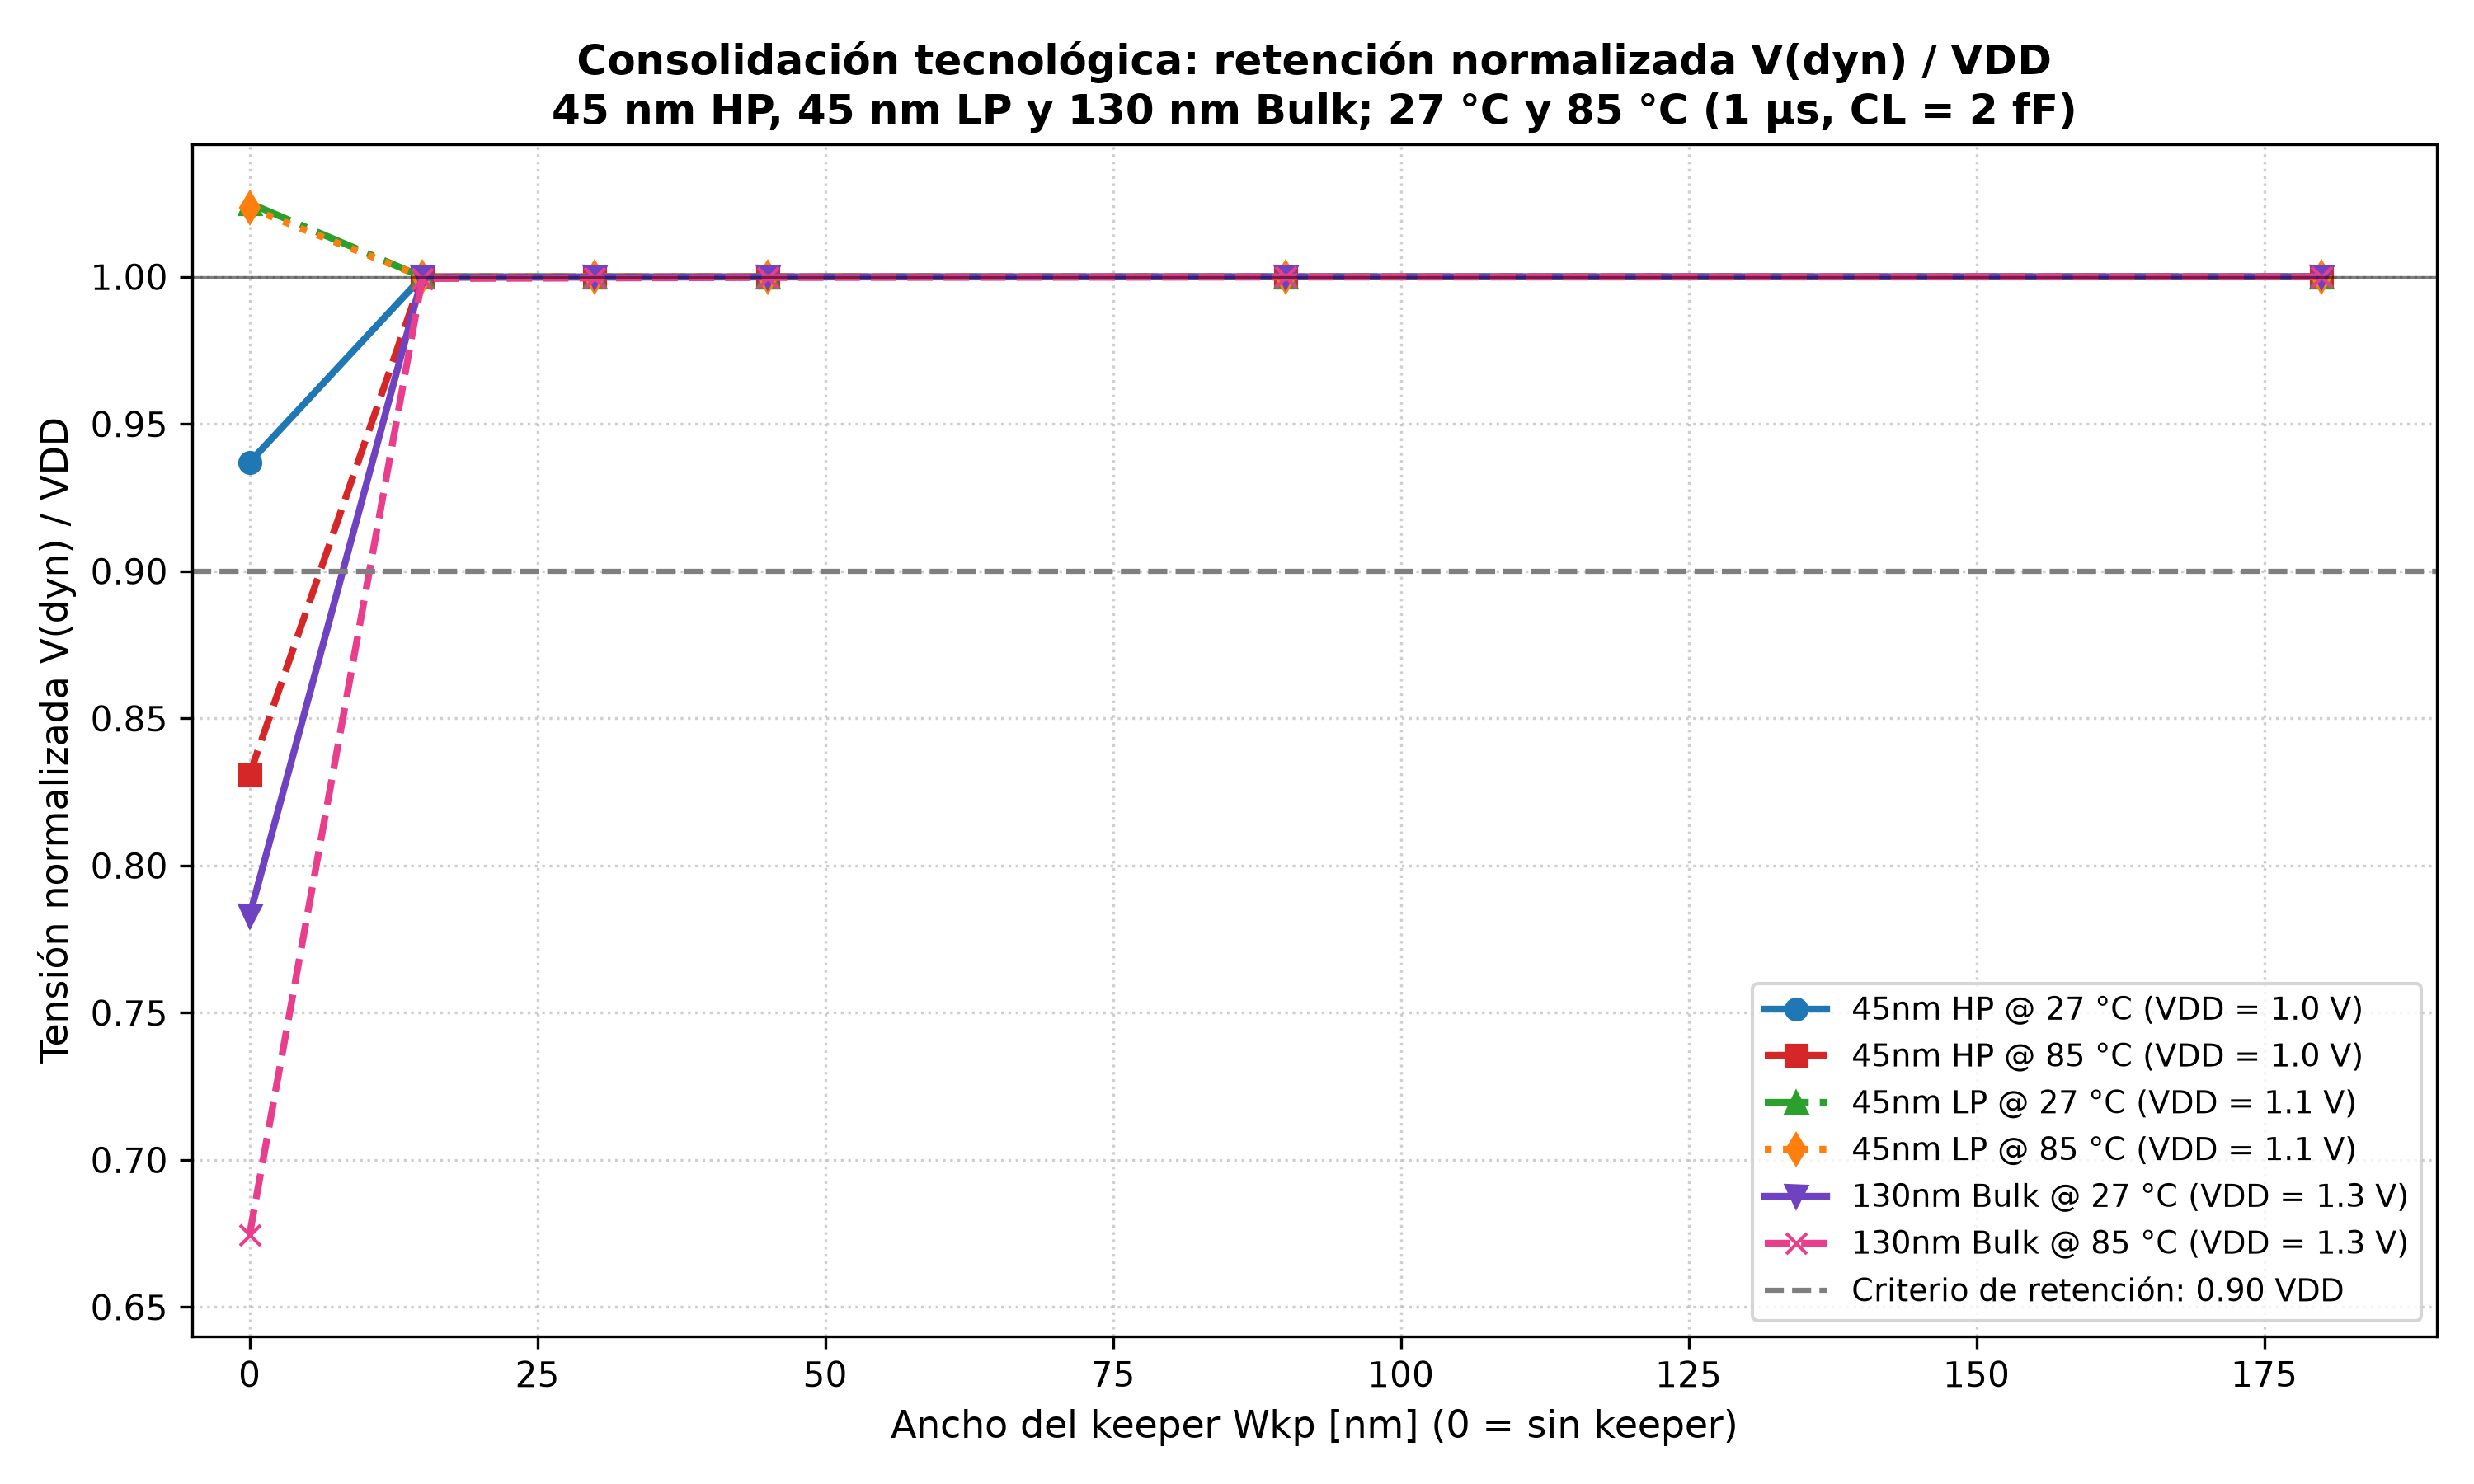
\includegraphics[width=0.78\linewidth]{figuras/fig2_act3_consolidacion_hp_lp_130.png}
  \caption[Consolidación tecnológica tri-nodo de retención]{Tensión normalizada de retención $V_{dyn}(1\,\mu\text{s})/V_{DD}$ en función de $W_{kp}$ para 45\,nm HP, 45\,nm LP y 130\,nm Bulk a $27^\circ\text{C}$ y $85^\circ\text{C}$ ($T_{\text{stop}}=1\,\mu\text{s}$).}
  \label{fig:consolidacion_tecnologica}
\end{figure}

\begin{enumerate}[leftmargin=1.4em,itemsep=0.15em]
  \item \textbf{Tecnología 45\,nm Low Power (LP, $V_{DD}=1.1\,\text{V}$):} Exhibe menor caída del nodo en este ensayo. El óxido de compuerta más grueso ($t_{oxe} = 1.80\,\text{nm}$) y el umbral nominal mayor ($V_{th0} \approx 0.62\,\text{V}$) contribuyen a reducir las fugas; a $85^\circ\text{C}$ se midieron $7.06\,\text{pA}$ de corriente media de alimentación y $3.40\,\text{pA}$ en la rama PDN (magnitudes distintas). El nodo termina en $1.1275\,\text{V}$ a $27^\circ\text{C}$ y $1.1257\,\text{V}$ a $85^\circ\text{C}$; la sobretensión inicial por acoplamiento no equivale a ganancia de carga neta. No requiere keeper para satisfacer el criterio en la ventana simulada de $1\,\mu\text{s}$ ($t_{\text{hold}} > 1.0\,\mu\text{s}$, formalmente censurado en $T_{\text{ret}} = 1000.0\,\text{ns}$).
  \item \textbf{Tecnología 130\,nm Bulk ($V_{DD}=1.3\,\text{V}$):} En la configuración ensayada, con $W_n = 3 \times 260\,\text{nm} = 780\,\text{nm}$ y $C_L=2\,\text{fF}$, la red presenta una descarga apreciable: cruza el umbral de $0.90\,V_{DD} = 1.17\,\text{V}$ en $t_{\text{cross}} = 318.83\,\text{ns}$ ($t_{\text{hold}} = 318.31\,\text{ns}$) a $27^\circ\text{C}$ y en $t_{\text{cross}} = 168.05\,\text{ns}$ ($t_{\text{hold}} = 167.53\,\text{ns}$) a $85^\circ\text{C}$. A $85^\circ\text{C}$ termina en $0.8770\,\text{V}$; aunque la salida no conmuta espuriamente ($V_M \approx 0.60\,\text{V}$), \textbf{falla el criterio estricto de retención}. El ancho $W_{kp} = 15.0\,\text{nm}$ es el menor punto ensayado en la malla de simulación que lo satisface, no un límite físico universal intrínseco. Asimismo, la comparación entre nodos involucra variaciones simultáneas en $W_n$ y $V_{DD}$, por lo que no aísla de forma exclusiva el efecto intrínseco de la tecnología.
\end{enumerate}

\noindent\textbf{Efecto del Keeper en 45\,nm HP:} La adición de un transistor PMOS gobernado por la salida restauradora $out$ sostiene el nodo flotante. En los anchos discretos ensayados entre $10.5$ y $180\,\text{nm}$ (incluido el punto de la guía $W_{kp}=22\,\text{nm}$), se obtiene $V_{dyn}(1\,\mu\text{s}) > 0.9999\,\text{V}$ a ambas temperaturas. No se ha demostrado retención ilimitada ni un ancho mínimo continuo. El valor $W_{kp} = 10.5\,\text{nm}$ corresponde a la cota inferior evaluada en la malla de simulación fina que converge y satisface retención; en el modelo BSIM4 PTM 45\,nm, el parámetro intrínseco $W_{\text{int}} = 5\,\text{nm}$ impone un ancho eléctrico efectivo $W_{\text{eff}} = W - 2 W_{\text{int}} = W - 10\,\text{nm}$, por lo que valores $W \le 10\,\text{nm}$ (e.g., $W_{kp} = 1\,\text{nm}$) generan $W_{\text{eff}} \le 0$ y provocan el aborto numérico inmediato del simulador. Dicho límite numérico del modelo no debe confundirse con una regla de diseño de fundición (DRC).

\subsection{Evaluación de Contención y Penalización de Velocidad en Evaluación Activa}
Aunque un keeper suficientemente dimensionado compensa la descarga por fugas durante la ventana simulada, su presencia introduce el fenómeno de \textbf{contención de corriente} (\textit{keeper contention}) durante la fase de evaluación activa ($CLK=1, A=B=C=1$). En el instante en que la PDN comienza a descargar el nodo dinámico, la salida del inversor dominó aún permanece en nivel bajo ($out = 0\,\text{V}$), manteniendo al keeper encendido. El keeper disputa corriente con los transistores NMOS en serie, inyectando portadores desde $V_{DD}$ y demorando la conmutación hacia tierra.

Conforme a la tarea~4 de la guía, se define una razón geométrica de dimensionamiento relativo $r$ que normaliza el ancho del keeper respecto al ancho equivalente de la red de descarga (PDN). En la tecnología 45\,nm HP, el ancho unitario de referencia es $W_{n,\text{unit}} = 90\,\text{nm}$. Para compensar la degradación por apilamiento, los transistores de la PDN se dimensionan a $W_{n,\text{stack}} = 3 \times W_{n,\text{unit}} = 270\,\text{nm}$. Dado que la PDN footed consta de 4 transistores NMOS en serie (tres de la compuerta lógica $M_1, M_2, M_3$ y el transistor footed de reloj $M_f$, todos con $W_n = 270\,\text{nm}$ y $L_n = 45\,\text{nm}$), el ancho equivalente de la pila en serie se aproxima geométricamente por:
\begin{equation}
  W_{PDN,eq} \approx \frac{W_{n,\text{stack}}}{4} = \frac{270\,\text{nm}}{4} = 67.5\,\text{nm}
\end{equation}
Adoptando longitudes nominales de canal idénticas ($L_p = L_n = 45\,\text{nm}$), la razón de aspecto de dimensionamiento resulta:
\begin{equation}
  r \equiv \frac{(W/L)_{kp}}{(W/L)_{PDN,eq}} = \frac{W_{kp}/L_p}{W_{PDN,eq}/L_n} = \frac{W_{kp}/45\,\text{nm}}{67.5\,\text{nm}/45\,\text{nm}} = \frac{W_{kp}}{67.5\,\text{nm}}
  \label{eq:ratio_r}
\end{equation}
Es fundamental precisar que $r$ constituye una métrica heurística y puramente geométrica de dimensionamiento relativo adoptada según la guía docente, y \textbf{no} un cómputo riguroso de la resistencia efectiva de conmutación o una extracción dinámica de pequeña señal (la cual se ve fuertemente afectada por la saturación de velocidad, el efecto de cuerpo variable $V_{SB} > 0$ a lo largo de la pila y las tensiones transitorias de sobremarcha $V_{GS} - V_{th}$).
La rúbrica docente fija como cota estricta que la penalización en el retardo de evaluación no debe exceder el 10\%:
\begin{equation}
  \text{Penalización } \Delta t_{pHL} \equiv \frac{t_{pHL,dyn}(W_{kp}) - t_{pHL,\text{base}}}{t_{pHL,\text{base}}} \times 100\% < 10.0\%
  \label{eq:cota_contencion}
\end{equation}
donde el retardo de referencia sin keeper a $85^\circ\text{C}$ es $t_{pHL,\text{base}} = 31.80\,\text{ps}$ en 45\,nm HP y $105.74\,\text{ps}$ en 45\,nm LP.

% Tabla de contencion y penalizacion de retardo en evaluacion - Actividad 3
% Fuentes: act3_contencion_metricas.json, act3_conciliacion_a3_5_1.json, act3_descomposicion_causal.json
\begin{table}[htbp]
\centering
\footnotesize
\caption[Penalización de velocidad por contención del keeper en evaluación activa]{Penalización de velocidad en evaluación activa ($A=B=C=1$) bajo peor caso térmico ($85^\circ\text{C}$, $C_L=2.0\,\text{fF}$, $C_{out}=1.0\,\text{fF}$).}
\label{tab:contencion}
\begin{tabularx}{\linewidth}{@{}>{\RaggedRight\arraybackslash}p{3.2cm} c c c c >{\RaggedRight\arraybackslash}X@{}}
\toprule
\textbf{Arquitectura / Configuración} & \textbf{$W_{kp}$} & \textbf{$r = \frac{W_{kp}}{67.5\,\text{nm}}$} & \textbf{$t_{pHL,dyn}$} & \textbf{Penaliz. $\Delta t_{pHL}$} & \textbf{Estado frente a Cota Estricta $< 10.0\%$} \\
\midrule
\multicolumn{6}{@{}l@{}}{\textbf{Tecnología 45\,nm HP ($V_{DD}=1.0\,\text{V}$, $t_{pHL,\text{base}} = 31.80\,\text{ps}$)}} \\
Sin Keeper (Referencia) & --- & --- & 31.80\,ps & 0.00\% & Referencia base inalterada. \\
Keeper Convencional (Mín. Malla) & 10.5\,nm & 0.156 & 32.96\,ps & +3.64\% & \textbf{CUMPLE}. Mínimo ensayado en la malla de simulación. \\
Keeper Convencional (Punto Guía §7) & 22.0\,nm & 0.326 & 33.47\,ps & +5.25\% & \textbf{CUMPLE}. Cumple holgadamente velocidad y retención. \\
Keeper Convencional (Frontera Máx.) & 38.0\,nm & 0.563 & 34.96\,ps & \textbf{+9.94\%} & \textbf{CUMPLE}. Máximo ancho ensayado que cumple velocidad (+9.96\% Config B). \\
Keeper Convencional (Primer Fallo) & 39.0\,nm & 0.578 & 35.09\,ps & \textbf{+10.35\%} & \textbf{FALLA}. Excede la cota estricta del 10.0\%. \\
Keeper Convencional Unitario & 45.0\,nm & 0.667 & 35.90\,ps & +12.90\% & \textbf{FALLA}. Inadmisible ($I_{kp,\max} = 17.65\,\mu\text{A}$). \\
Keeper Convencional Límite & 180.0\,nm & 2.667 & $\infty$ & $\infty$ & \textbf{FALLA SEVERA}. Pérdida de conmutación ($V_{dyn,\min}=0.633\,\text{V} > V_M$). \\
\midrule
\multicolumn{6}{@{}l@{}}{\textbf{Tecnología 45\,nm LP ($V_{DD}=1.1\,\text{V}$, $t_{pHL,\text{base}} = 105.74\,\text{ps}$)}} \\
Keeper LP (Frontera Máxima) & 36.0\,nm & 0.533 & 116.30\,ps & \textbf{+9.99\%} & \textbf{CUMPLE}. Máximo ensayado admisible en LP. \\
Keeper LP (Primer Fallo) & 37.0\,nm & 0.548 & 116.78\,ps & \textbf{+10.45\%} & \textbf{FALLA}. Excede la cota estricta del 10.0\%. \\
\midrule
\multicolumn{6}{@{}l@{}}{\textbf{Alternativa Complementaria: Keeper Condicional (45\,nm HP @ $85^\circ\text{C}$)}} \\
Control 2 PMOS Serie ($\tau=0\,\text{ps}$) & 45.0\,nm & 0.667 & 33.61\,ps & +5.69\% & \textbf{CUMPLE}. $I_{kp,\max}=9.38\,\mu\text{A}$, solapamiento de 52\,ps. \\
Keeper Condicional con 3 Inv. & 45.0\,nm & 0.667 & 33.43\,ps & \textbf{+5.11\%} & \textbf{CUMPLE}. $I_{kp,\max}=9.40\,\mu\text{A}$, solapamiento acortado a 44\,ps. \\
\bottomrule
\end{tabularx}
\end{table}


\begin{figure}[htbp]
  \centering
  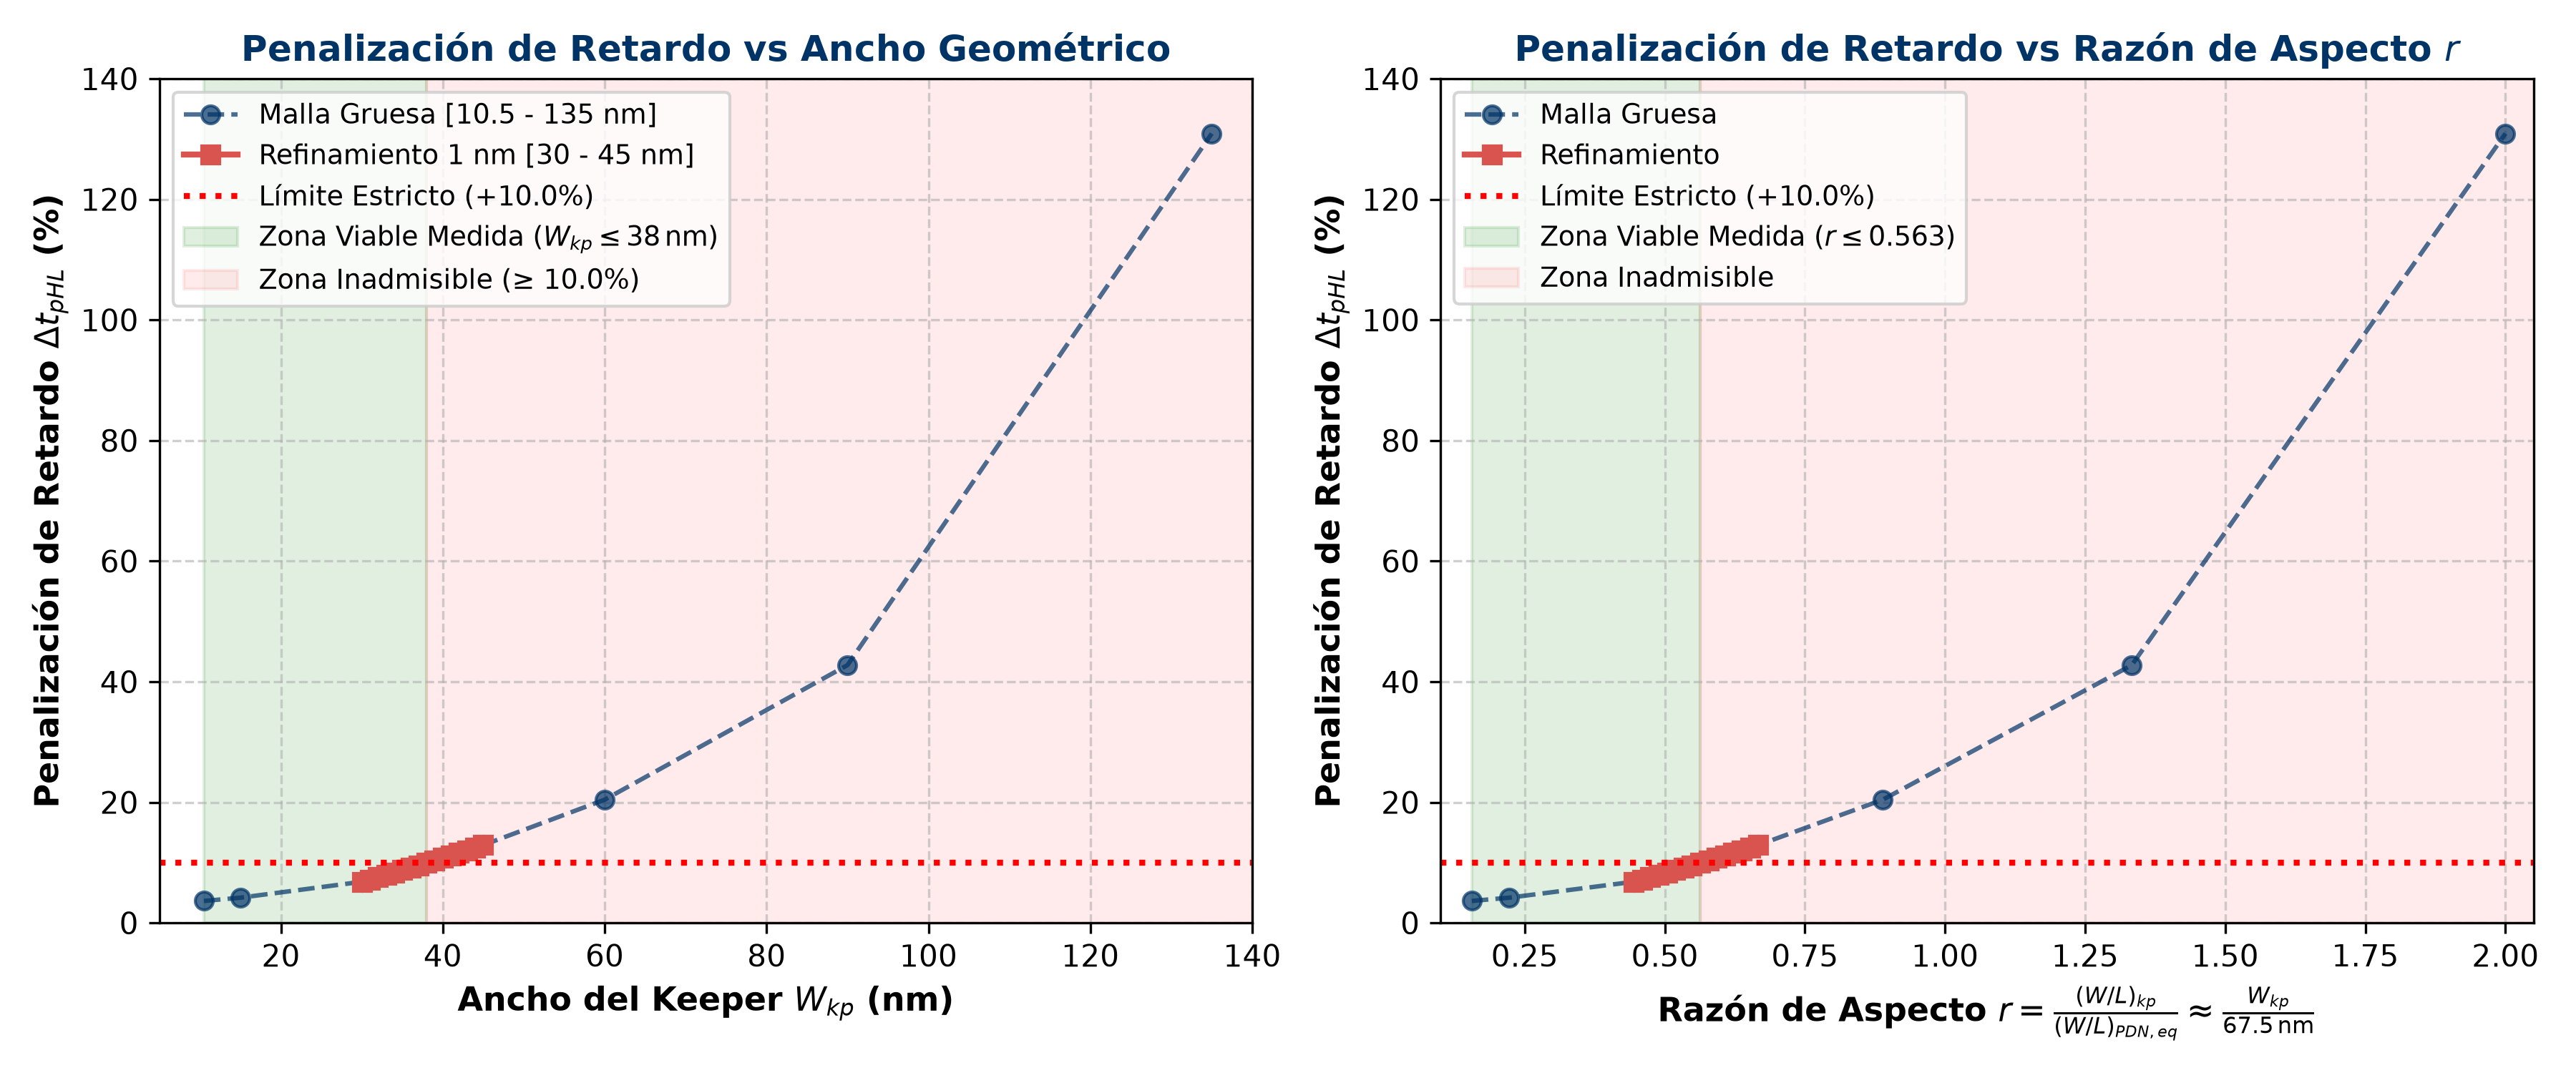
\includegraphics[width=0.68\linewidth]{figuras/fig3_act3_contencion_penalizacion.png}
  \caption[Penalización de retardo vs ancho del keeper y razón de aspecto]{Penalización porcentual del retardo de evaluación $\Delta t_{pHL}$ en función de $W_{kp}$ y de la razón de aspecto $r$ (45\,nm HP @ $85^\circ\text{C}$), identificando la malla gruesa y el refinamiento de 1\,nm en la frontera del 10.0\%.}
  \label{fig:contencion_penalizacion}
\end{figure}

Los resultados cuantitativos se exponen en la Tabla~\ref{tab:contencion} y en la Figura~\ref{fig:contencion_penalizacion}:
\begin{itemize}[leftmargin=1.4em,itemsep=0.15em]
  \item \textbf{Frontera Crítica en 45\,nm HP @ $85^\circ\text{C}$:} 
  \begin{itemize}[leftmargin=1.2em,itemsep=0.08em]
    \item $W_{kp} = 38.0\,\text{nm}$ ($r = 0.563$): es el \textbf{máximo ancho ensayado que satisface la cota de velocidad}, registrando $t_{pHL} = 34.96\,\text{ps}$ ($\Delta t_{pHL} = \mathbf{+9.94\%}$ bajo Configuración A y $\mathbf{+9.96\%}$ bajo Configuración B de alta precisión numérica).
    \item $W_{kp} = 39.0\,\text{nm}$ ($r = 0.578$): es el primer ancho ensayado que \textbf{incumple la cota}, alcanzando $\Delta t_{pHL} = \mathbf{+10.35\%}$.
    \item Un keeper convencional unitario ($W_{kp} = 45\,\text{nm}$, $r = 0.667$) induce una degradación inadmisible de $+12.90\%$ ($t_{pHL} = 35.90\,\text{ps}$), drenando una corriente de pico de contención de $I_{kp,\max} = 17.65\,\mu\text{A}$.
    \item Para anchos desmedidos ($W_{kp} = 180\,\text{nm}$, $r = 2.667$), la contención impide que la PDN descargue el nodo ($V_{dyn,\min} = 0.633\,\text{V} > V_M$), provocando una falla lógica catastrófica por pérdida total de conmutación.
  \end{itemize}
  \item \textbf{Frontera Crítica en 45\,nm LP @ $85^\circ\text{C}$:} Debido a la menor corriente de saturación de la PDN, el límite estricto se desplaza a $W_{kp} = 36.0\,\text{nm}$ ($r = 0.533$), el cual cumple con $\Delta t_{pHL} = \mathbf{+9.99\%}$ ($116.30\,\text{ps}$), mientras que $37.0\,\text{nm}$ supera el umbral con $\mathbf{+10.45\%}$.
\end{itemize}

\subsection{Compromiso Retención/Velocidad y Ventana de Viabilidad Conjunta}
La intersección simultánea de ambos requerimientos define la \textbf{ventana de viabilidad conjunta}:
\begin{equation}
  \mathcal{W}_{\text{viable}} = \left\{ W_{kp} \in \mathbb{R}^+ \;:\; V_{dyn}(1.0\,\mu\text{s}) \ge 0.90\,V_{DD} \quad \land \quad \Delta t_{pHL}(W_{kp}) < 10.0\% \right\}
\end{equation}

\begin{figure}[htbp]
  \centering
  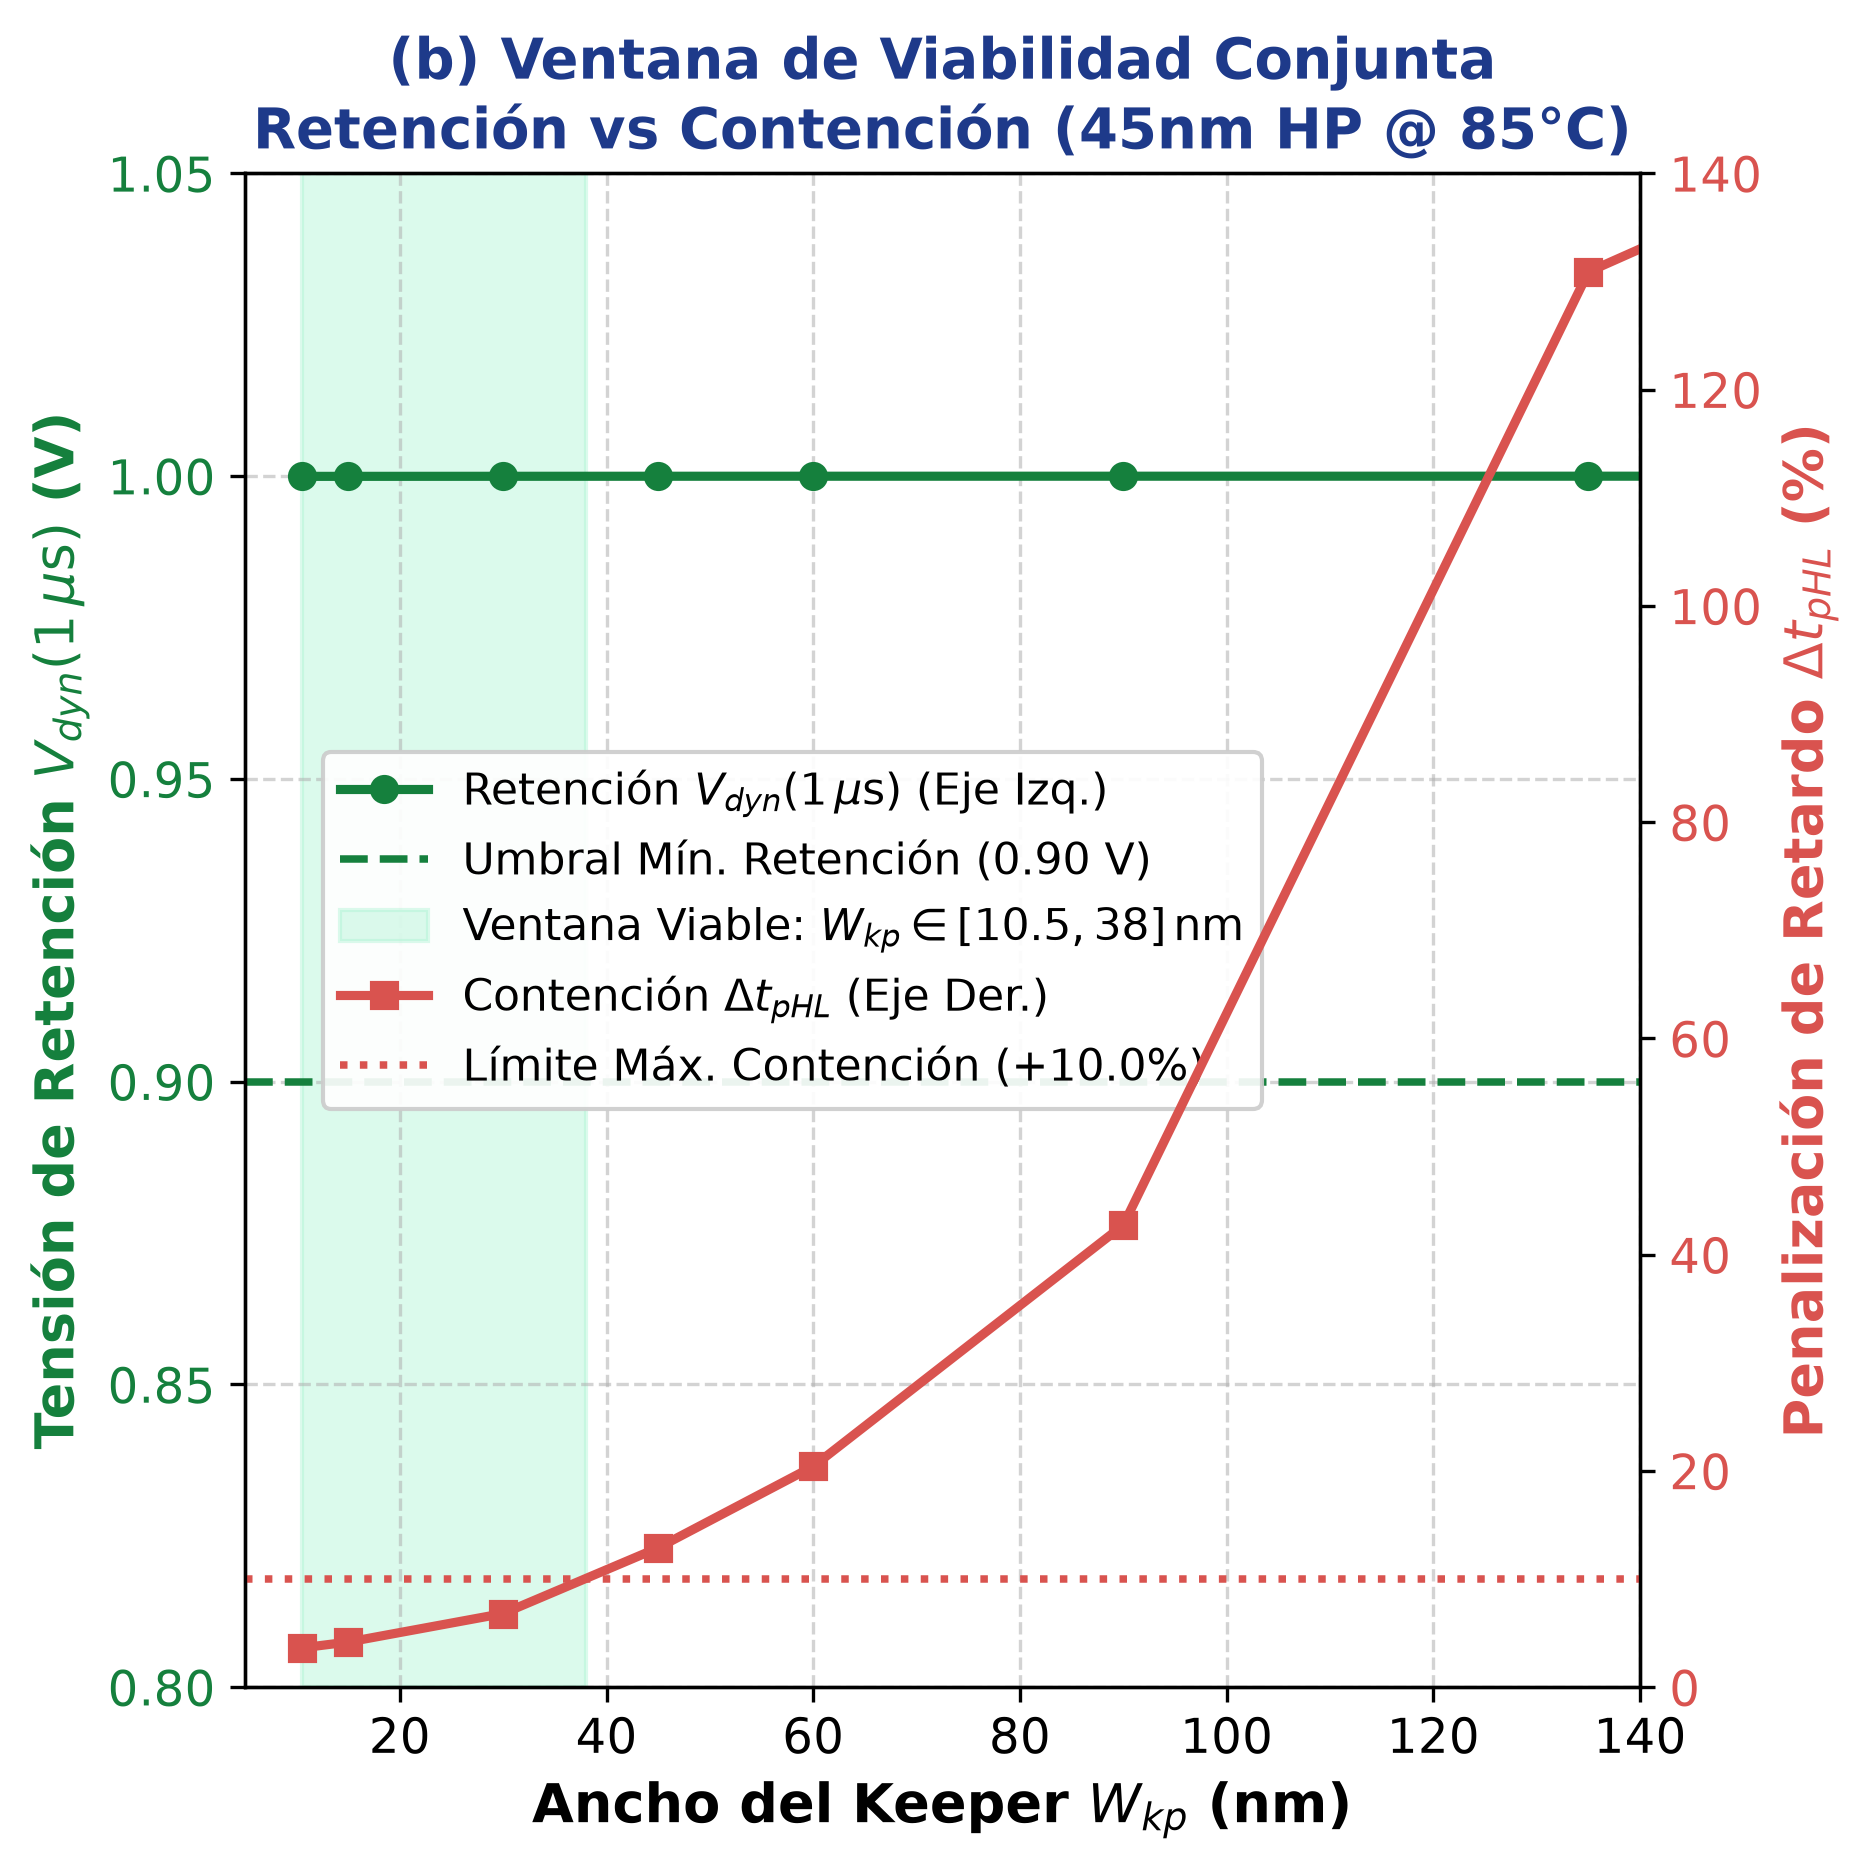
\includegraphics[width=0.62\linewidth]{figuras/fig4_act3_ventana_viabilidad.png}
  \caption[Ventana de viabilidad conjunta retención vs contención]{Ventana de viabilidad conjunta retención vs contención para la NAND3 en 45\,nm HP a $85^\circ\text{C}$. Los puntos de retención entre 31\,nm y 34\,nm se infieren a partir de la tendencia observada en los puntos simulados y la monotonicidad teórica esperada de la corriente del keeper con el ancho de canal, mientras que los valores de contención provienen de simulación transitoria directa.}
  \label{fig:ventana_viabilidad}
\end{figure}

Como se ilustra en la Figura~\ref{fig:ventana_viabilidad}, en 45\,nm HP a $85^\circ\text{C}$, la ventana viable delimitada sobre la malla de simulación comprende:
\begin{equation}
  W_{kp} \in [10.5\,\text{nm},\; 38.0\,\text{nm}] \quad \iff \quad r \in [0.156,\; 0.563]
\end{equation}
\noindent\textbf{Delimitación Metodológica de Evidencia Directa e Inferida:}
El respaldo experimental sobre la malla ensayada distingue tres regímenes: (1)~\textbf{Puntos viables con simulación directa completa}: los anchos $W_{kp} = 10.5$, $15$, $22$, $30$, $35$, $36$, $37$ y $38\,\text{nm}$ cuentan con simulaciones independientes de retención durante $1.0\,\mu\text{s}$ y de retardo activo, verificando simultáneamente ambos criterios con una penalización máxima de $\mathbf{+9.94\%}$ en $38\,\text{nm}$. (2)~\textbf{Punto de control externo de frontera}: $W_{kp} = 39\,\text{nm}$, ensayado directamente en ambos requisitos, queda fuera de la ventana viable al identificar el primer incumplimiento estricto de velocidad ($\Delta t_{pHL} = \mathbf{+10.35\%}$). (3)~\textbf{Retención inferida}: para los anchos intermedios $W_{kp} = 31$, $32$, $33$ y $34\,\text{nm}$, la contención proviene de simulación transitoria directa en malla de $1\,\text{nm}$, mientras que la retención durante $1\,\mu\text{s}$ se infiere por la monotonicidad teórica de la corriente restauradora y la cota observada en los extremos simulados ($V_{dyn} > 0.9999\,\text{V}$ en $30$ y $35\,\text{nm}$).

Por consiguiente, la ventana viable $[10.5,\, 38.0]\,\text{nm}$ queda demostrada empíricamente sobre la malla ensayada, sin postular continuidad analítica universal para todo valor intermedio ni reglas de diseño de fabricación (DRC) comerciales.

\subsection{Alternativas de Diseño: Keeper Condicional con Línea de Retardo}
La respuesta a la tarea~5 de la guía confirma que, aunque existe una ventana viable en 45\,nm HP, esta se encuentra restringida a anchos sub-micrométricos estrechos ($W_{kp} \le 38\,\text{nm}$). Un diseñador que restrinja el keeper al transistor unitario de referencia cuadrada ($W = L = 45\,\text{nm}$), adoptado como cota de dimensionamiento frente a anchos sub-litográficos sin respaldo de reglas DRC comerciales, queda automáticamente fuera de la especificación de velocidad ($\Delta t_{pHL} = +12.90\%$, con $t_{pHL} = 35.90\,\text{ps}$).

Para superar esta limitación, se implementó y ensayó la arquitectura de \textbf{Keeper Condicional} en el marco de este proyecto. La topología reemplaza el transistor simple por dos dispositivos PMOS en serie ($W = 45\,\text{nm}$ cada uno):
\begin{itemize}[leftmargin=1.4em,itemsep=0.12em]
  \item $M_{k,fb}$: Conectado al nodo dinámico $dyn$, gobernado por la salida $out$ como lazo de realimentación.
  \item $M_{k,en}$: Conectado a $V_{DD}$, gobernado por una señal de habilitación retrasada $CLK_{\text{del}}$ generada por una cadena de 3 inversores estáticos ($W_n = 90\,\text{nm}, W_p = 135\,\text{nm}$, retardo $\tau_{\text{del}} \approx 16.15\,\text{ps}$).
\end{itemize}

\begin{figure}[htbp]
  \centering
  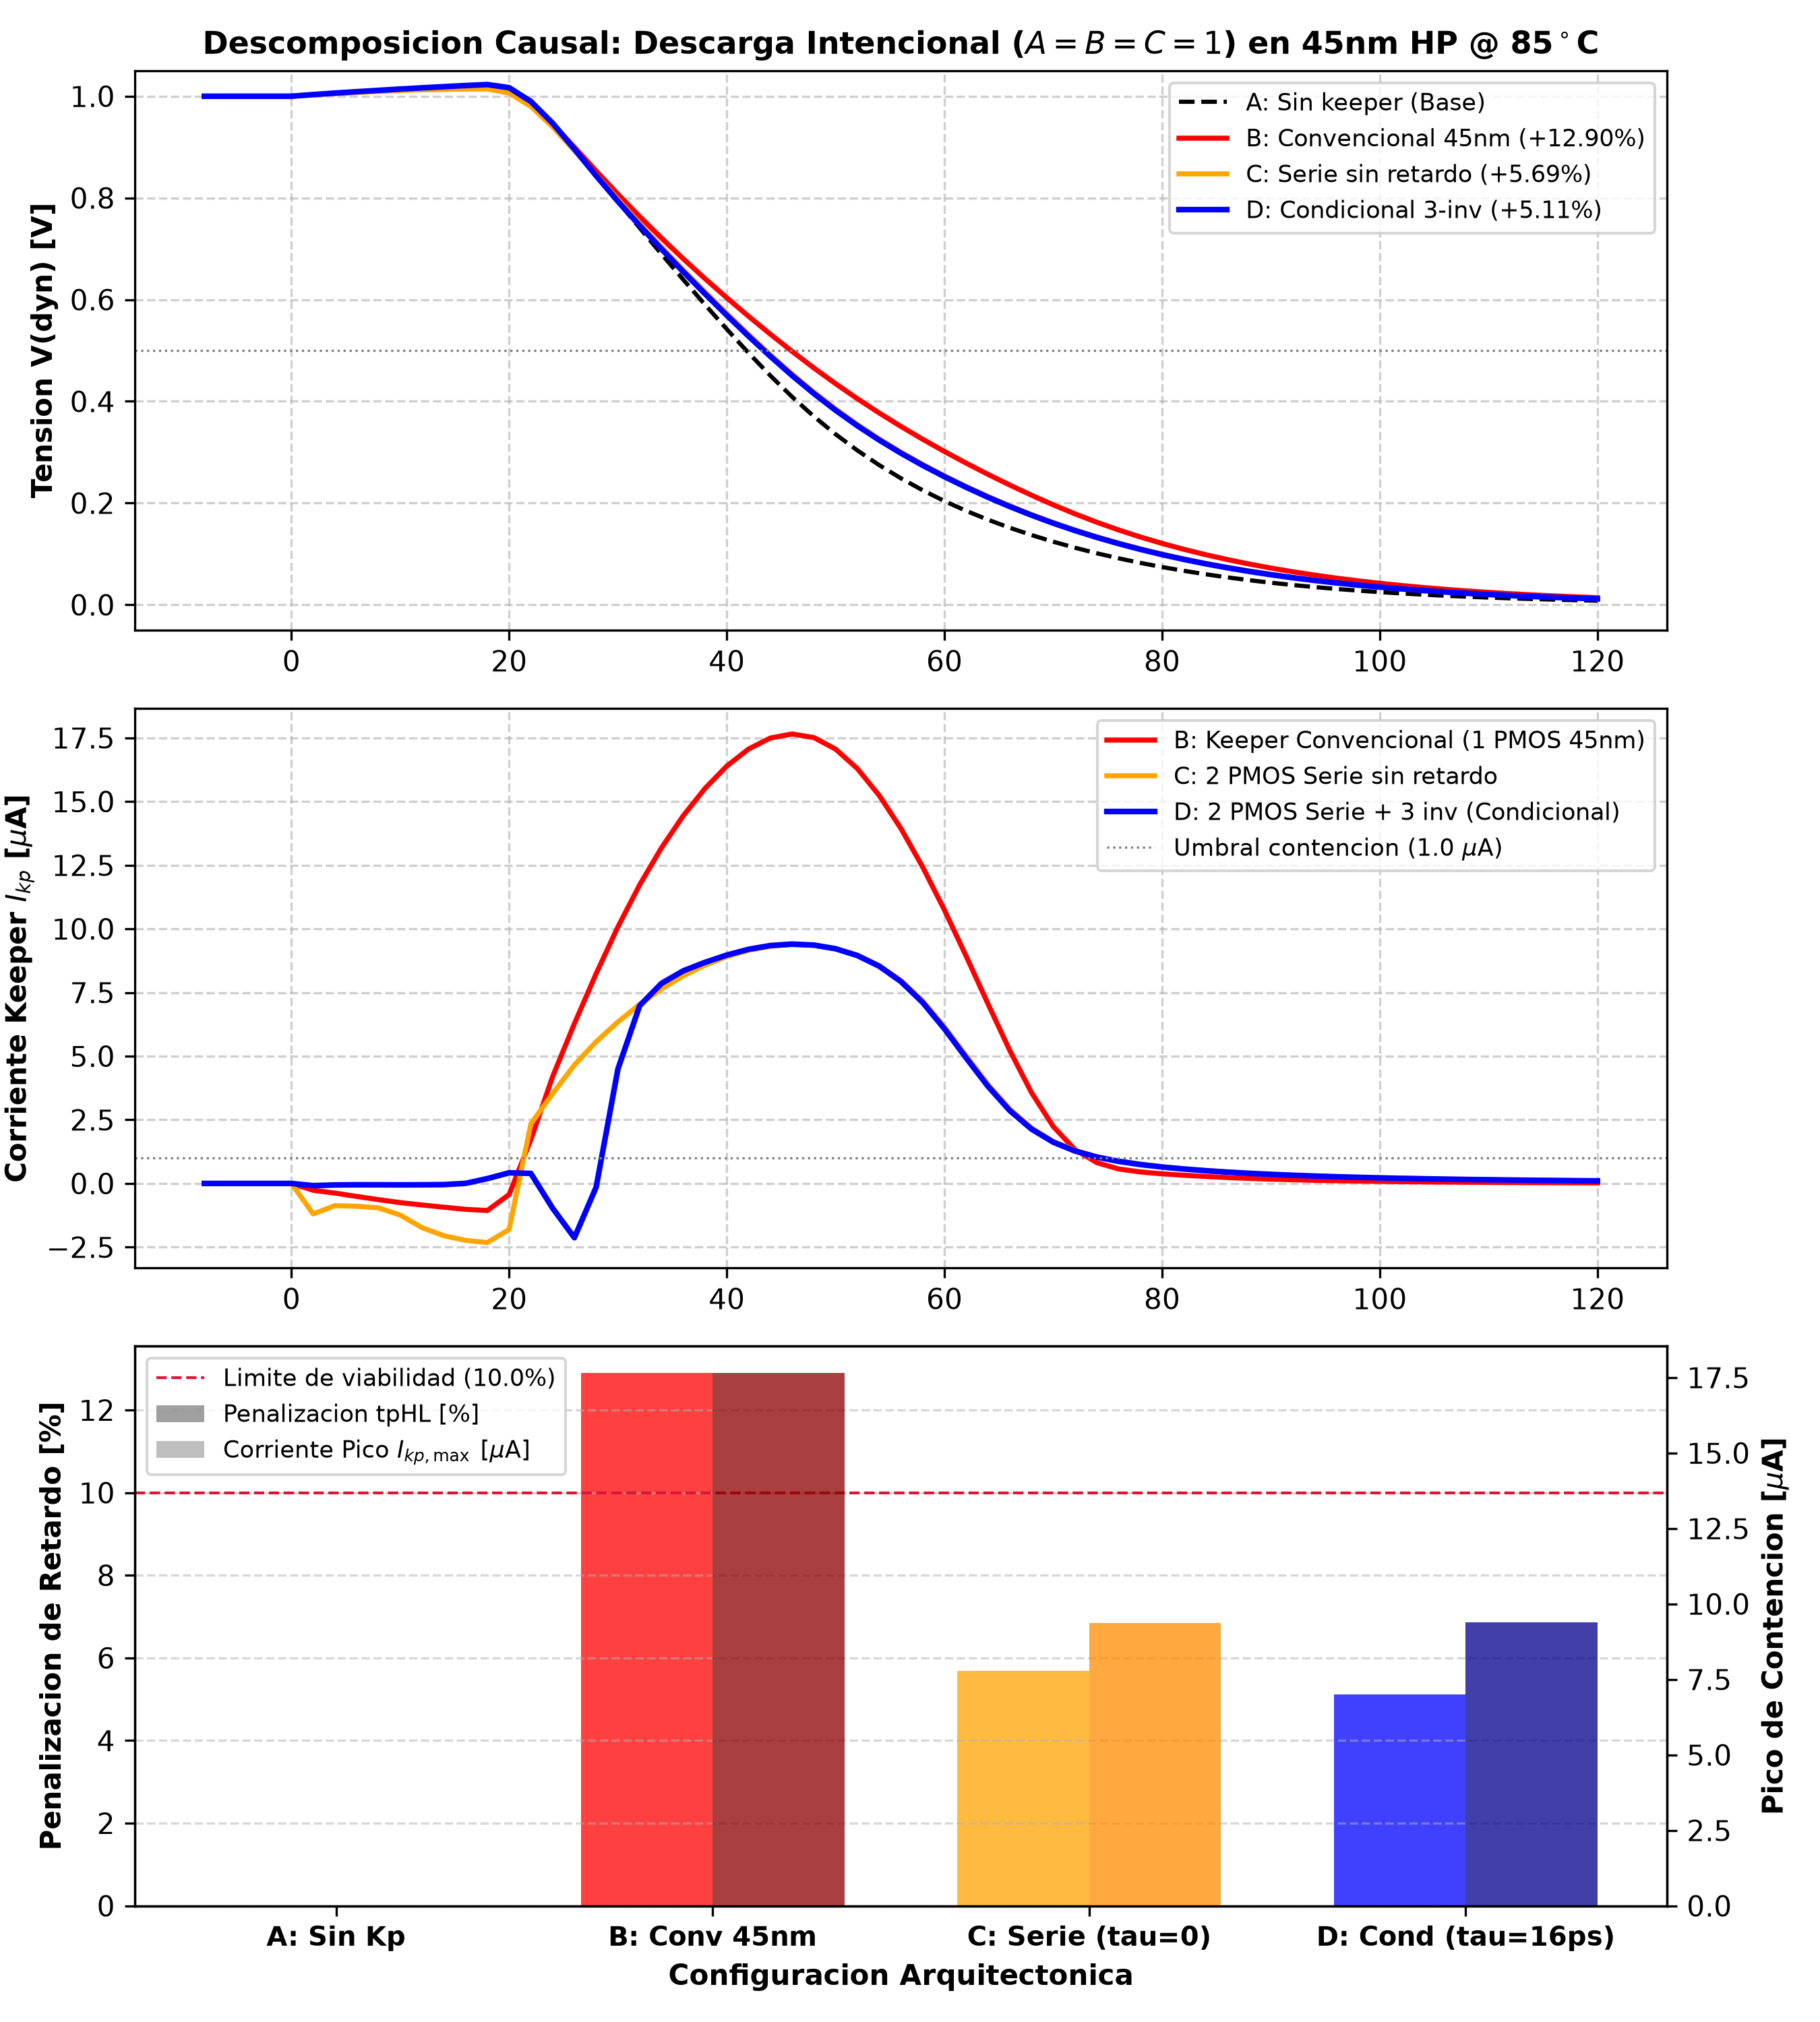
\includegraphics[width=0.62\linewidth]{figuras/fig5_act3_keeper_condicional.png}
  \caption[Descomposición causal del keeper condicional]{Descomposición causal del transitorio de evaluación activa ($A=B=C=1$) en 45\,nm HP a $85^\circ\text{C}$, comparando las formas de onda $V(dyn)$, la corriente instantánea de contención $I_{kp}(t)$ y la penalización de retardo.}
  \label{fig:keeper_condicional}
\end{figure}

La Figura~\ref{fig:keeper_condicional} detalla la respuesta transitoria y la corriente instantánea de contención, contrastando cuatro arquitecturas:
\begin{enumerate}[leftmargin=1.4em,itemsep=0.15em]
  \item \textbf{A (Sin Keeper):} Referencia base ideal sin contención ($t_{pHL} = 31.80\,\text{ps}$).
  \item \textbf{B (Keeper Convencional de 45\,nm):} Fuerte contención con pico $I_{kp,\max} = 17.65\,\mu\text{A}$, extendiéndose durante $50.0\,\text{ps}$ (intervalo de solapamiento $t \in [22.0,\, 72.0]\,\text{ps}$) y penalizando el retardo en $\mathbf{+12.90\%}$ ($35.90\,\text{ps}$).
  \item \textbf{C (Control de 2 PMOS Serie Síncronos, $\tau=0\,\text{ps}$):} Al disponer dos PMOS en serie comandados síncronamente, la duplicación de la resistencia de canal abate el pico de corriente a $9.38\,\mu\text{A}$ (reducción de 46.9\%), reduciendo la penalización a $\mathbf{+5.69\%}$ ($33.61\,\text{ps}$) con una duración de solapamiento de $52.0\,\text{ps}$ ($t \in [22.0,\, 74.0]\,\text{ps}$).
  \item \textbf{D (Keeper Condicional con 3 Inversores de Retardo):} La cadena retardada introduce un desfase en el inicio de la contención ($t_{\text{start}} = 22.0 \to 30.0\,\text{ps}$) y anticipa el corte del keeper respecto a la descarga de $dyn$, reduciendo la duración del solapamiento de contención a $44.0\,\text{ps}$ ($t \in [30.0,\, 74.0]\,\text{ps}$). La penalización cae a $\mathbf{+5.11\%}$ ($33.43\,\text{ps}$).
\end{enumerate}

\noindent\textbf{Causalidad Física No Lineal y Rol del Retardo:} Es imperativo destacar la explicación física subyacente: en la configuración con cadena de retardo se observa simultáneamente una menor \textbf{duración temporal} del solapamiento de contención (de $52.0\,\text{ps}$ en C a $44.0\,\text{ps}$ en D, frente a $50.0\,\text{ps}$ en B) y una menor penalización de retardo (+5.69\% $\to$ +5.11\%), sin que se reduzca el valor pico de corriente de contención ($I_{kp,\max}$ pasa de $9.38\,\mu\text{A}$ a $9.40\,\mu\text{A}$, con una variación menor al $0.3\%$ atribuible a acoplamientos parásitos de compuerta). Si bien la reducción del tiempo de conflicto disminuye el intervalo durante el cual el keeper disputa portadores contra la red de descenso, no debe atribuirse causalidad exclusiva a dicho recorte temporal sin un experimento de ablación que desacople completamente el retardo de la conmutación de los transistores y las cargas nodales internas.

\noindent\textbf{Compromiso de Sobrecarga de Reloj (\textit{Clock Overhead}):} La inclusión del primer inversor de retardo agrega la capacitancia de su compuerta ($W_n=90\,\text{nm}, W_p=135\,\text{nm} \implies C_g \approx 0.279\,\text{fF}$) a la red de distribución de reloj, la cual originalmente excitaba únicamente a $M_p$ y $M_f$ ($C_{clk,\text{base}} \approx 0.503\,\text{fF}$). Esto representa un incremento puramente geométrico de área de compuerta estimado en $\Delta C_{clk}/C_{clk,\text{base}} \approx \mathbf{+55.5\%}$.

\noindent\textbf{Validación de Inmunidad y Robustez:}
\begin{itemize}[leftmargin=1.4em,itemsep=0.1em]
  \item \textbf{Retención Estática ($1.0\,\mu\text{s}$):} En reposo ($CLK=1, A=B=C=0$), la salida del tercer inversor se fija en nivel bajo permanente, manteniendo habilitado el keeper condicional y garantizando $V_{dyn}(1\,\mu\text{s}) = 1.0000\,\text{V}$ sin caída.
  \item \textbf{Recuperación frente a Compartición de Carga ($CLK=1, A=B=1, C=0$):} Sometido al peor caso de compartición (Actividad~2), el nodo experimenta una caída inicial a $V_{dyn,\min} = 0.9247\,\text{V}$ ($\Delta V = 75.3\,\text{mV}$); el keeper condicional restaura el potencial dinámico hasta $0.9980\,\text{V}$ antes de culminar la evaluación, asegurando que la salida se mantenga inmutable ($V_{out} < 0.18\,\text{mV}$).
\end{itemize}

En las condiciones y tiempos ensayados, el keeper condicional permite usar transistores de $45\,\text{nm}$ y cumplir simultáneamente la retención durante la ventana ensayada de $1\,\mu\text{s}$ y el límite de penalización de velocidad del 10\%. No se postula retención ilimitada; su comportamiento a escalas temporales mayores requeriría modelamiento adicional de fugas en reposo prolongado.
